\chapter{Writing USB Drivers}
\label{chap:usb-drivers}

This chapter provides documentation and general guidelines for usage of the
refactored USB device driver interface. As such, it is meant for developers of
HelenOS device drivers, who can use it as a reference guide. By intention, this
section abstracts the reader from all modifications to the stack, and focuses
only on the latest state of the interface. All changes to the interface are
described in detail in Chapter \ref{usb-refactoring}.

The reader should note that there exists a similar section in the initial USB
stack documentation. The text in this chapter could be considered an updated
version or extension of that text.


\section{Basics}

This section gives details on the basic structure of USB device drivers, their
role in the system and components they usually interact with.


\subsection{Framework}

USB device drivers use the generic \textit{Device Driver Framework} available in
HelenOS. Because all USB drivers have similar initialization routines, a thin
layer -- specific to USB devices -- was added above the generic one. This layer
mainly serves as a middleware for easy communication with USB host controller
drivers, performing USB specific resource management and enabling device drivers
to initialize endpoint pipes and interact with USB devices. For those reasons,
USB device drivers are recommended to link with \lib{libdrv} and
\lib{libusbdev}, which contain both aforementioned layers respectively.

It is expected that USB device drivers specify in advance not only their
relevant match identifiers, which are used by the Device Manager to pair new
devices with available drivers, but also all endpoints, which shall be present
on the device through a USB driver structure. Later when a new device is found,
a specialized device structure is prepared and pipe abstractions are
initialized.

Device drivers live the same life cycle as any other drivers controlled by the
\textit{Device Manager}. A quick summary follows:
~
\begin{enumerate}
	\item The driver is started at the convenience of the Device Manager if and
	when a compatible device is found. At startup, the driver registers with the
	USB framework, which in turn registers also with the Device Driver
	Framework.

	\item During its lifetime, the driver receives callbacks from the USB
	Framework, informing it about relevant device events. On the basis of these
	events, the driver then communicates with the device and exposes various
	interfaces to other tasks in the system. At this point, the controlled
	device usually becomes visible and useful to the user.

	\item When there is no more need for the driver to run (i.e. no devices to
	control), the Device Manager may terminate the driver to save resources.
\end{enumerate}

In the Device Driver Framework, drivers are the consumers of \textit{devices}
and providers of \textit{functions}. This paradigm allows them to expose an
unlimited number of nodes (representing logical or physical units) for every
device they control. The same basic principle holds for USB drivers as well.


\subsection{Device Callbacks}

As explained in the previous section, USB device drivers are informed about
relevant device events by asynchronous callbacks from the USB framework. To
simplify usage, these callbacks are identical to those of the Device Driver
Framework:
~
\begin{description}
	\item[Add Device] This event notifies the driver that a new device has been
	discovered and matched to it. From this point on, the driver is allowed to
	communicate with the device in order to configure it and expose its
	functions to the rest of the system. Further communication with the device
	will likely depend on remote calls originating from other system tasks
	utilizing the exposed interface.

	\item[Remove Device] This event instructs the driver to immediately disallow
	new user operations on a device, terminate all currently running
	operations in a timely manner, and hand device control back to the system,
	as the device will likely be physically removed from the bus in the
	forseeable future.

	\item[Device Gone] This event informs the driver that a device has been
	physically disconnected from the system without a prior \textit{Remove
	Device} event. Since the device is no longer reachable, the driver is to
	force interrupt all user operations, which were running at the time of
	receiving the event and report failure to the callers.
	
	\item[Offline Function] By receiving this event, the driver is asked by the
	system to explicitly transition a specific function exposed by one of its
	controlled devices into the \textit{Offline} state. The meaning of such
	transition might depend on the interpretation of the function. For more
	information, see the Device Driver Framework Documentation.

	\item[Online Function] By receiving this event, the driver is asked by the
	system to explicitly transition a specific function exposed by one of its
	controlled devices into the \textit{Online} state. Again, the meaning of such
	transition might depend on the interpretation of the function. For more
	information, see the Device Driver Framework Documentation.
\end{description}

\begin{figure}
	\centering
	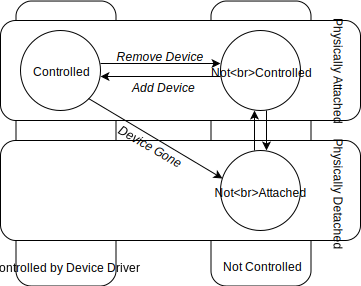
\includegraphics[width=0.5\textwidth]{device-states}
	\caption[Diagram of USB device states and transition events.]{Diagram of USB
	device states and transition events, as perceived by the device driver. Note
	that these states do \textit{not} correspond to USB bus device states (e.g.
	\textit{Configured}, \textit{Addressed}, etc.) in any way.}
	\label{fig:device-states}
\end{figure}

The listed events are delivered to device drivers through function calls to
event handlers specified in the main USB driver operations structure (see
Listing \ref{lst:driver-ops-structure} for a minimal example). The order of
event delivery models the physical lifecycle of the device within the system.
For instance, it is not possible for the \textit{Add Device} event to occur more
than once for the same device in a row. For reference, the exact device states
and transitions between them (corresponding to the events with respective names)
are shown in Figure \ref{fig:device-states}.

Furthermore, since there are no guarantees on the synchronization between calls,
the driver is explicitly responsible for synchronizing accesses to its private
data structures as well as device communication.

\begin{listing}
	\begin{code}
		static int device_add(usb_device_t *dev)
		{
			usb_log_info("Device '%s' added.", usb_device_get_name(dev));
			return EOK;
		}

		static int device_remove(usb_device_t *dev)
		{
			usb_log_info("Device '%s' removed.", usb_device_get_name(dev));
			return EOK;
		}

		static int device_gone(usb_device_t *dev)
		{
			usb_log_info("Device '%s' gone.", usb_device_get_name(dev));
			return EOK;
		}

		static const usb_driver_ops_t driver_ops = {
			.device_add = device_add,
			.device_remove = device_remove,
			.device_gone = device_gone,
		};
	\end{code}
	\caption[Main USB device driver operations structure.]{Main USB device
	driver operations structure with corresponding event handlers. Note that
	events \textit{Offline Function} and \textit{Online Function} do not require
	a handler and can therefore be omitted in the minimal example.}
	\label{lst:driver-ops-structure}
\end{listing}


\section{Device Communication}

In USB, \textit{a pipe} is an abstraction primitive for a communication channel
between a device and a host computer. For the sake of simplicity, the provided
framework relies on a mechanism based on the same abstraction in order to
facilitate communication between device drivers and devices.


\subsection{Endpoint Description}

In order to use pipes, device drivers must first define at least one
\textit{endpoint description}. The purpose of such definition is to specify all
device endpoints, which will be used for communication by the device driver
throughout its lifecycle. For that reason, all descriptions ought to be
specified in advance and referenced in the main device driver structure (for
example of possible endpoint description definition, refer to Listing
\ref{lst:driver-ep-array}).

\begin{listing}
	\begin{code}
		static const usb_endpoint_description_t bulk_in_ep = {
			.transfer_type = USB_TRANSFER_BULK,
			.direction = USB_DIRECTION_IN,
			.interface_class = USB_CLASS_MASS_STORAGE,
			.interface_subclass = USB_MASSSTOR_SUBCLASS_SCSI,
			.interface_protocol = USB_MASSSTOR_PROTOCOL_BBB,
			.flags = 0
		};

		static const usb_endpoint_description_t bulk_out_ep = {
			.transfer_type = USB_TRANSFER_BULK,
			.direction = USB_DIRECTION_OUT,
			.interface_class = USB_CLASS_MASS_STORAGE,
			.interface_subclass = USB_MASSSTOR_SUBCLASS_SCSI,
			.interface_protocol = USB_MASSSTOR_PROTOCOL_BBB,
			.flags = 0
		};

		static const usb_endpoint_description_t *endpoints[] = {
			&bulk_in_ep, &bulk_out_ep, NULL
		};
	\end{code}
	\caption[Main USB device driver endpoint description array]{Main USB device
	driver endpoint description array. This particular example shows two
	\textit{Bulk} endpoints for SCSI mass storage data transfers in both the
	\textit{In} and \textit{Out} directions.}
	\label{lst:driver-ep-array}
\end{listing}

Endpoint description contains information which can be matched to USB endpoint
descriptors in very much the same way as match identifiers are used to pair
devices with device drivers in HelenOS. Following this scheme, the presented USB
framework does most of the heavy lifting for device drivers. When a new device
is added, prior to delivery of the \textit{Add Device} event, all endpoint
descriptions provided by the driver are matched to device endpoints, resulting
in two possible outcomes for every description:
~
\begin{enumerate}
	\item A device endpoint matching the provided description is found and
		\textit{an endpoint mapping} is created.
	\item No device endpoint matches the provided description, hence no mapping is
		created.
\end{enumerate}

Device drivers can later query the result of the matching, and if successful,
retrieve the created endpoint mapping containing a fully initialized pipe
instance. An example of this is shown in Listing \ref{lst:driver-ep-mapping}.

\begin{listing}
	\begin{code}
		static int device_add(usb_device_t *dev)
		{
			/* Find mapping for the endpoint description. */
			usb_endpoint_mapping_t *mapping = usb_device_get_mapped_ep_desc(dev, &bulk_out_ep);

			/* Determine if the mapping was successful. */
			if (!mapping || !mapping->present) {
				usb_log_error("Endpoint mapping failed!");
				return ENOENT;
			}

			usb_pipe_t *pipe = &mapping->pipe;

			/* Now we can write to `pipe`. */
			return write_data(pipe);
		}
	\end{code}
	\caption[Obtaining USB pipe from an endpoint description.]{Sample
	implementation of the \textit{Device Add} event handler, obtaining a mapping
	and a USB pipe from one endpoint description defined in Listing
	\ref{lst:driver-ep-array}.}
	\label{lst:driver-ep-mapping}
\end{listing}

\subsection{Pipe I/O}

Provided that an endpoint description has been defined, successfully matched
and an endpoint mapping has been retrieved along with a pipe instance, a device
driver can schedule data transfers to a device.

Pipes offer a very simple synchronous command interface similar to that of an
open file descriptor, namely \fnc{usb_pipe_read} and \fnc{usb_pipe_write} for
reading from \textit{In} endpoints and writing to \textit{Out} endpoints
respectively. While semantics of these functions depends on endpoint types
(consult USB specification for details), their basic usage is as follows:
~
\begin{enumerate}
	\item Device driver allocates a buffer of appropriate size (and fills it
		with data if writing).
	\item Either the \fnc{usb_pipe_read} or \fnc{usb_pipe_write} function is
		called, scheduling transfers to the device. The function receives a pipe
		pointer, pointer to the user-allocated buffer and data size.
	\item The calling fibril is blocked until transfers succeed or fail (see
		error code). If reading, the number of read bytes is returned as well.
	\item Device driver recycles or disposes of the allocated buffer.
\end{enumerate}

Note that while the write function blocks the calling fibril until the entire
buffer is transferred to the device, the read function might return successfully
with a lower number of bytes read than the actual data size requested, and may
thus have to be called multiple times.

In addition, due to multiplatform nature of HelenOS, it is not advisable to
assume endianity of the host system. Instead, the \macro{uint{16|32}_host2usb}
and \macro{uint{16|32}_usb2host} macros serve to convert host system endianity
to and from the transfer endianity defined in the USB Protocol Specification at
driver's convenience. A complete example of pipe write is shown in Listing
\ref{lst:pipe-write}.

\begin{listing}
	\begin{code}
		static int write_data(usb_pipe_t *pipe)
		{
			int rc = EOK;
			/* Allocate memory. */
			static const size_t size = 64;
			char *buffer = (char *) malloc(size);
			if (!buffer) {
				rc = ENOMEM;
				goto err;
			}

			/* Fill `buffer` with arithmetic sequence of bytes. */
			for (int i = 0; i < size; ++i) buffer[i] = (char) i;

			/* Write data. */
			rc = usb_pipe_write(pipe, buffer, size);
			if (rc != EOK) {
				usb_log_error("Write failed with error: %s", str_error(rc));
				goto err_buffer;
			}

			/* Clean up. */
		err_buffer:
			free(buffer);
		err:
			return rc;
		}
	\end{code}
	\caption[Example write to a USB pipe.]{Example write to a USB pipe. This is
	a possible implementation of the \fnc{write_data} function referenced in
	Listing \ref{lst:driver-ep-mapping}.}
	\label{lst:pipe-write}
\end{listing}


\subsection{Automated Polling}

In USB devices which often interact with a human user, it is important to wait
for user input by spinning (or polling) on some \textit{Interrupt In} endpoint.
In the abstraction used, this translates to calling \fnc{usb_pipe_read} in a
perpetual loop and responding to incoming data or errors. Since this behavior is
common to a significant class of drivers, a reusable unified implementation is
provided by the USB framework.

The implementation is represented by the \struct{usb_polling_t} structure and
its associated functions. Similarly to device event handlers, device drivers are
expected to configure this structure with polling handler functions. Later when
polling should be initiated, a call to the \fnc{usb_polling_start} function will
spawn a separate fibril, spinning on the pipe and calling handlers when data
arrive or \fnc{usb_pipe_read} fails with error.

When polling is to be ceased, a call to the \fnc{usb_polling_join} function will
spontaneously wake up the polling fibril and block the caller fibril until its
termination. If polling is started, a call to this function must \textit{always}
occur no later than in the \textit{Remove Device} or \textit{Device Gone} event
handler in order to prevent the fibril from outlasting the device lifecycle
within driver private data structures..

Furthermore, note that once any device driver starts polling on a pipe, it
transfers the pipe ownership to the polling fibril, relinquishing all control
over it. That prohibits subsequent calls to \fnc{usb_pipe_read} or other
relevant functions. It is also not feasible to poll only for a limited time
period, then join and reuse the pipe for arbitrary data reads. This is due to
the fact that once \fnc{usb_polling_join} is called, the pipe is left closed for
all communication, destroying the underlying endpoint mapping.

An example usage of the pipe polling interface is shown in Listing
\ref{lst:polling-example}.


\section{Miscellaneous}

This section features general suggestions and recommendations for USB device
driver implementation.


\subsection{Device-specific Data Structures}

Device drivers often need to maintain stateful and descriptive information
related to their controlled devices. A common practice is to store this kind of
information in device-specific data structures. As their name suggests, such
structures usually correspond to a single controlled device, and can thus
closely follow its lifecycle, being allocated and configured when the device is
added and being freed upon its removal.

The presented USB framework offers device drivers a straightforward mechanism to
associate any of their data structures with USB devices by specifying custom
\textit{device data} in the \struct{usb_device_t} structure, which is present in
all device-related events. Device data is allocated at most once for every
device and can have any driver-specified, albeit constant size. When the device
is later removed from the driver, device data is automatically freed if present.

Allocation of device data is performed by a call to the
\fnc{usb_device_data_alloc} function. This function has the same return value
and semantics as the \fnc{calloc} function. In addition, the pointer returned by
this function is stored within the \struct{usb_device_t} structure and can be
retrieved from that point onward until the device is removed by a call to the
\fnc{usb_device_data_get} function. Example usage of this mechanism can be seen
in Listing \ref{lst:device-data-example}.

\begin{listing}
	\begin{code}
		typedef struct my_data {
			/* Any device-specific data here. */
			usb_polling_t polling;
		} my_data_t;

		static int device_add(usb_device_t *dev)
		{
			/* Allocate device data. */
			my_data_t *data = (my_data_t *) usb_device_data_alloc(dev, sizeof(my_data_t));
			if (!data) {
				return ENOMEM;
			}

			usb_polling_init(&data->polling);
			/* ... configure polling ... */
			usb_polling_start(&data->polling);

			return EOK;
		}

		static int device_remove(usb_device_t *dev)
		{
			/* Retrieve device data. */
			my_data_t *data = (my_data_t *) usb_device_data_get(dev);

			/* Stop polling. */
			usb_polling_join(&data->polling);
			usb_polling_fini(&data->polling);

			/* After returning, device data is freed automatically. */
			return EOK;
		}
	\end{code}
	\caption[Example device data allocation and usage.]{Example device data
	allocation and usage. In this case, the \struct{my_data_t} device-specific
	data structure is used to keep track of automated pipe polling. Not that
	some error conditions have been intentionally ignored for the sake of brevity.}
	\label{lst:device-data-example}
\end{listing}


\subsection{Logging}

Another useful feature of the USB device driver framework is a set of logging
macros. These macros copy the scheme common to the HelenOS logging framework,
offering various log levels a format string syntax for a variable number of
arguments consistent with the \fnc{printf} function syntax. With decreasing
severity, the presented logging macros are named as follows:
~
\begin{description}
	\item[\macro{usb_log_fatal}] for fatal errors,
	\item[\macro{usb_log_error}] for recoverable errors,
	\item[\macro{usb_log_warning}] for warnings,
	\item[\macro{usb_log_info}] for informational messages (produces a log
		message of the \textit{Note} level),
	\item[\macro{usb_log_debug}] for debugging messages,
	\item[\macro{usb_log_debug2}] for verbose debugging messages.
\end{description}

Prior to printing the first log message, the \fnc{log_init} function must be
called. During runtime, the default HelenOS log level can be adjusted by a
call to the \fnc{logctl_set_log_level} function. Keep in mind that in the
current implementation of HelenOS, every call to a logging macro results in a
IPC call. For that reason, it is not advisable to perform logging in
performance-sensitive parts of code, even if the log level is sufficiently high.

For more information about logging in HelenOS, consult the HelenOS
Documentation.


\subsection{Exposing an Interface}

In order for controlled hardware to become usable to system tasks, HelenOS
device drivers can expose IPC interfaces to abstract hardware-specific features
and provide a set of well-defined logical operations for device interaction.

In HelenOS IPC, one of the preferred ways to achieve this is by interacting with
\textit{services} -- system tasks, which run as daemons, and whose purpose is to
connect user tasks with device drivers. Since services usually keep track of
devices of the same category, it is necessary to first identify the appropriate
service for a driver and consult its documentation.

While the specifics of exposing IPC interfaces may vary for different device
categories, the general scheme remains the same:
~
\begin{enumerate}
	\item For a DDF function, fill a specific structure with configuration and
		call handlers Then register them with the respective system service.
	\item Respond to service-specific calls in compliance with service
		specification. Handling of these calls will likely result in
		communication with the device.
	\item When the device is removed, cease handling service calls and
		unregister the device from the service.
\end{enumerate}


\subsection{Descriptors}




